\documentclass[border=2mm]{standalone}
\usepackage{tikz}
\usepackage{graphicx}

% Define common parameters
\newcommand{\imgwidth}{2cm}
\newcommand{\imgheight}{2cm}

% Define styles
\tikzset{
ssvep label/.style={above},
ssvep arrow/.style={ultra thick, ->},
image node/.style={above, midway, inner sep=0},
}

\begin{document}
\begin{tikzpicture}[xscale=2, yscale=1.5]
            
   \draw [color=white, ultra thick]
    (0,-0.125) node[above] {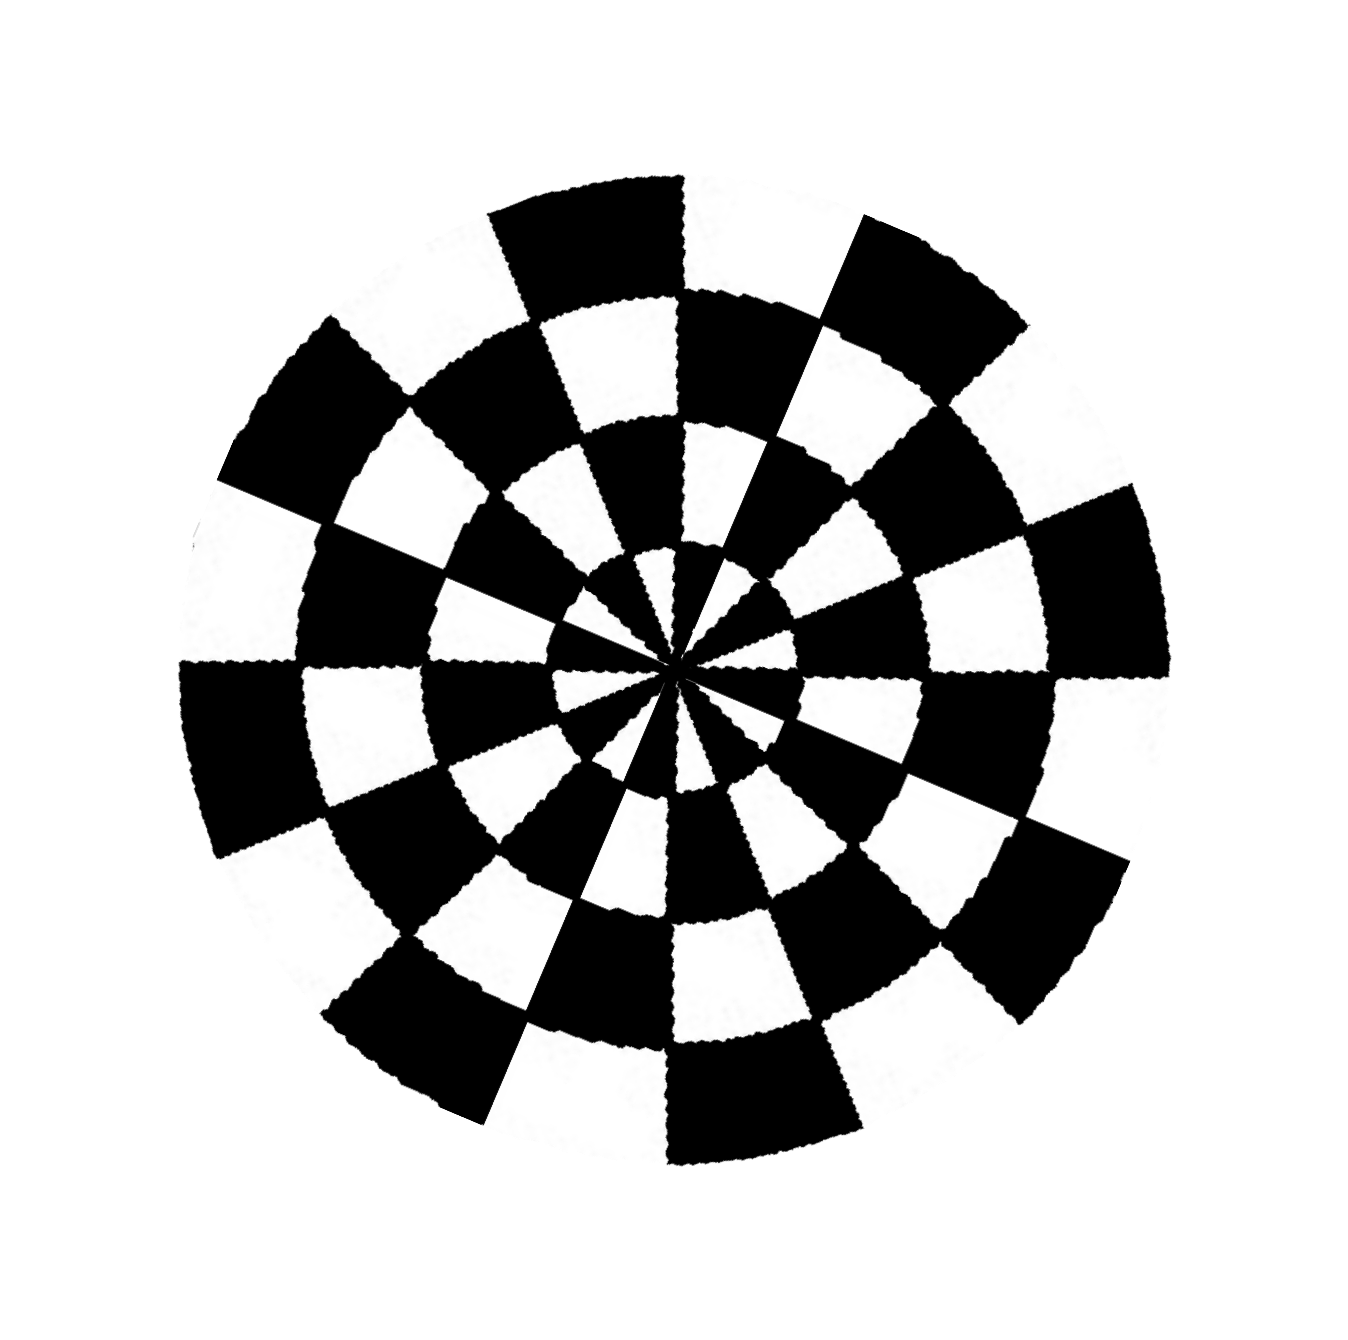
\includegraphics[width=2cm,height=2cm]{experiments/pattern.png}} 
    (1.5,-0.125) node[above] {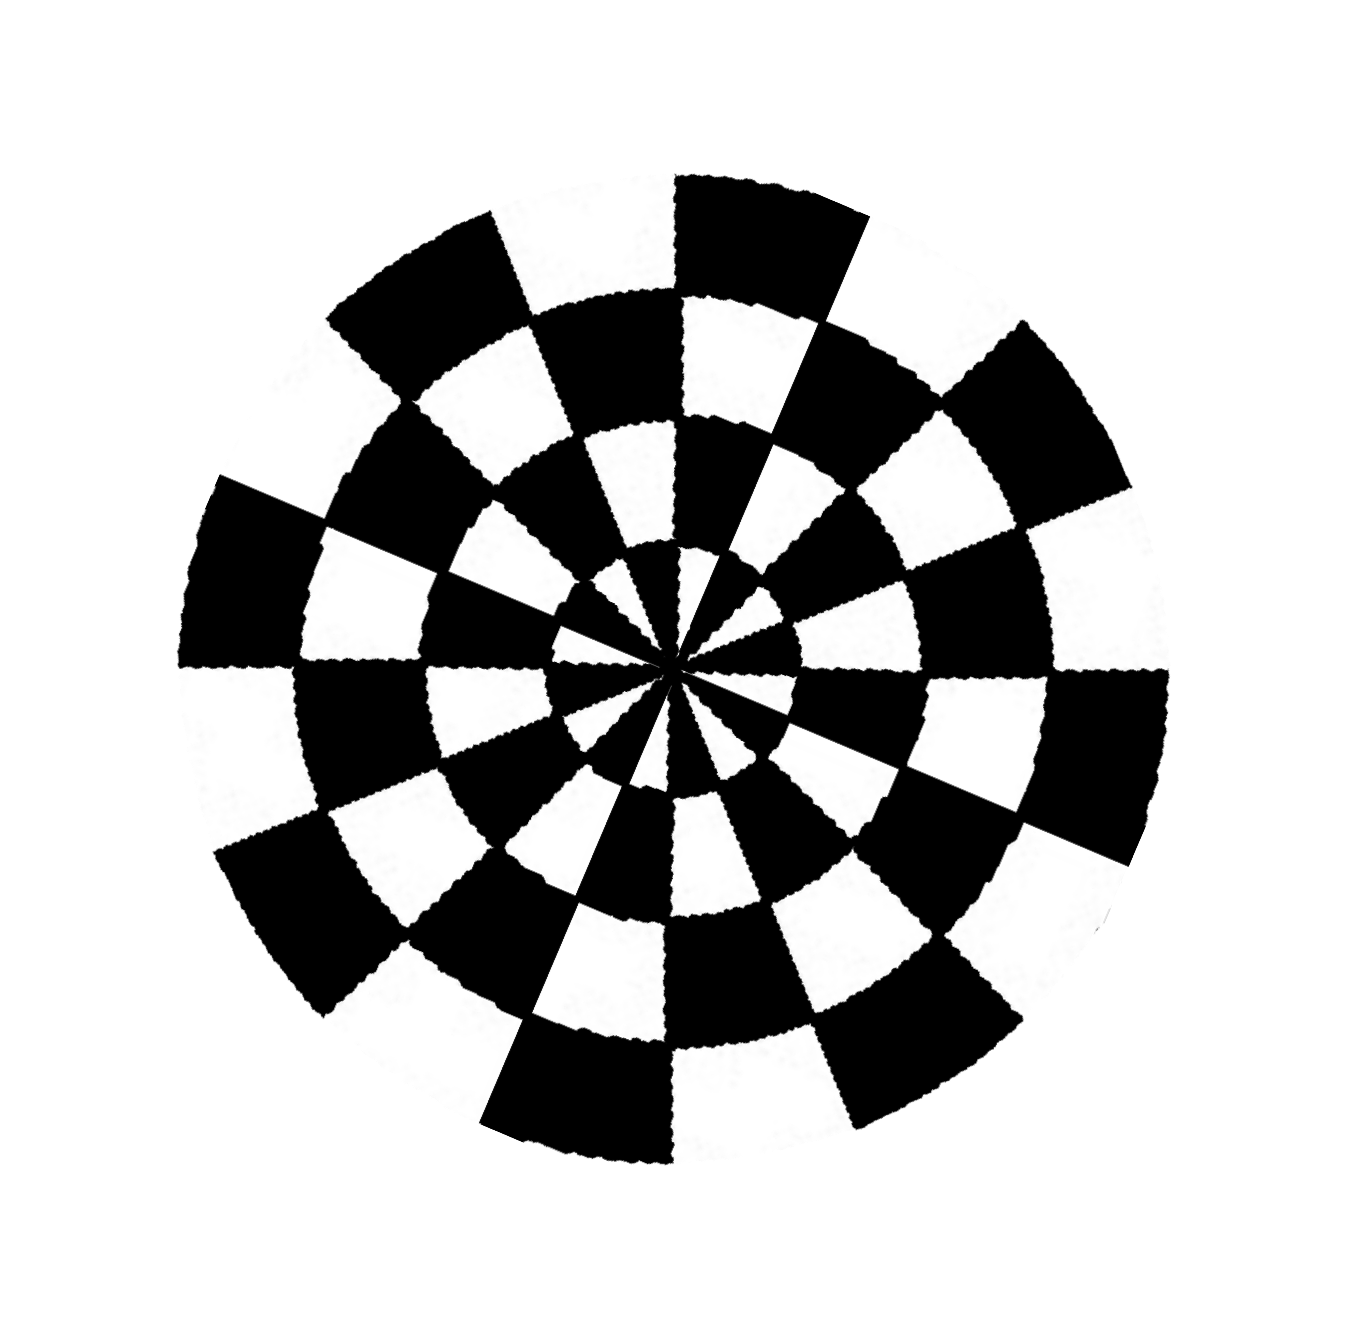
\includegraphics[width=2cm,height=2cm]{experiments/pattern_f.png}}
    ;
    
    % add SSVEP label on top of arrow
    \node[above] at (0.75,0.8-0.125) {6.6 Hz};
    \draw[ultra thick, <->] (0.5,0.75-0.125) -- (1,0.75-0.125);
    
  % draw vertical lines
    \foreach \i in {0,1,...,7} {
        \draw [thick] ({1.5*\i/8+2+0.5},0.5) -- ({1.5*\i/8+2+0.5},1);
    }

    
    % draw horizontal lines to form square wave
    \foreach \i in {0,1,...,7} {
        % check if i is even
        \ifodd\i
            \draw [thick] ({1.5*\i/8+2+0.5},0.5) -- ({1.5*(\i+1)/8+2+0.5},0.5);
        \else
            \draw [thick] ({1.5*\i/8+2+0.5},1) -- ({1.5*(\i+1)/8+2+0.5},1);
        \fi
    }
    
    % add line from (3,0) to (4.2,0)
    \draw [ultra thick, ->] (2+0.5,0.25) -- (4,0.25);
    \draw [ultra thick, ->] (2+0.5,0.25) -- (2+0.5,1.25);
    \node at (3.25, 0) {time (s)};
    \node at (2.5, 0) {0};
    \node at (4, 0) {1.2};
    \node at (2.2, 0.6) {min};
    \node at (2.2, 1) {max};
    
\end{tikzpicture}
\end{document}